%   %==========================================================================
%   %  Section
%   %==========================================================================
    \section{古典物理学の限界}
            \begin{mycomment}
                古典物理学の問題点は,先にあげた原子構造のほかに,固体比熱の問題と黒体輻射の問題が
                ある.固体比熱の問題は「熱・統計物理学」の部分で考えることにして,ここでは,黒体輻射
                    \footnote{
                        「空洞輻射」,「黒体放射」ともよばれる.
                    }
                の問題について考えることにする.
            \end{mycomment}

%       %======================================================================
%       %  Subsection
%       %======================================================================
            \subsection{黒体}
                \textbf{黒体} とはその名の通り,真っ黒な物体である.真っ黒な物体は,色付きの物体と
                違って,全ての電磁波を吸収する
                    \footnote{
                        色つきの物体は一部の色を吸収しその他を反射することで色を出しているのだ.
                    }.
                つまり,どの電磁波も吸収するということで,その意味で偏りのない物体である.また,こ
                ような黒体はそれ自身が熱をもちはじめると,発光し始める.黒体から発光される光は全て
                の波長の電磁波をふくみ,白っぽく光る.もちろん最初は赤い色を発光し,徐々に温度が高
                くなるに連れて光は青色に変化し,最終的に白くなるということである.

                マクスウェルの電磁波理論より,光の色は電磁波の波長 $\nu$ によって決まることがわかる.こ
                の周波数 $\nu$ のときの光の強度を $u(\nu)$ と表現する.
                すると,光の強度 $u(\nu)$ はどのような関数だろうかという疑問が生じるが,古典論から
                光の強度 $u(\nu)$ の具体的な形を導こうとしても,実験と完全に一致する式を導出するこ
                とはなかなかできなかった.以下に実験結果の例を示しておく
                    %\footnote{
                    %    関根 松夫 著,『量子電磁気学』,コロナ社,1996,p7より.
                    %}.

                キルヒホッフ
                    \footnote{
                        Gustav Robert Kirchhoff (1824‐1887,)
                    }
                は

%       %======================================================================
%       %  Subsection
%       %======================================================================
        \subsection{黒体輻射}
            一般に固体は温度を上げていくと赤く光り,さらに温度を上げていくと,しだいに白い光を発す
            るようになる.この現象は \textbf{黒体輻射} とよばれる.
                \begin{figure}[hbt]
                    \begin{center}
                        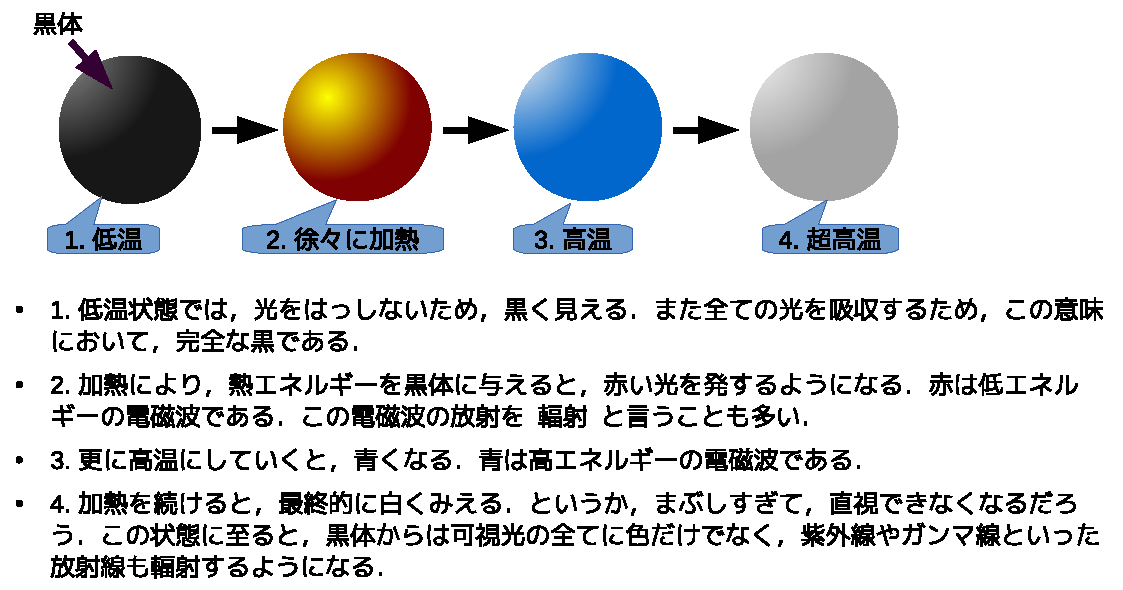
\includegraphics[keepaspectratio, width=7cm,height=5cm,clip]{KokutaiHoushaHakkou1111.pdf}
                        \caption{黒体輻射}
                        \label{fig:kokutai_housha_1}
                        \end{center}
                \end{figure}

            ここで問題とするのは,物体の発する光の色 と そのときの光の強度 の関係で
            ある.実験によれば,図\ref{fig:kokutai_housha_1}のようになる.
                \begin{figure}[hbt]
                    \begin{center}
                        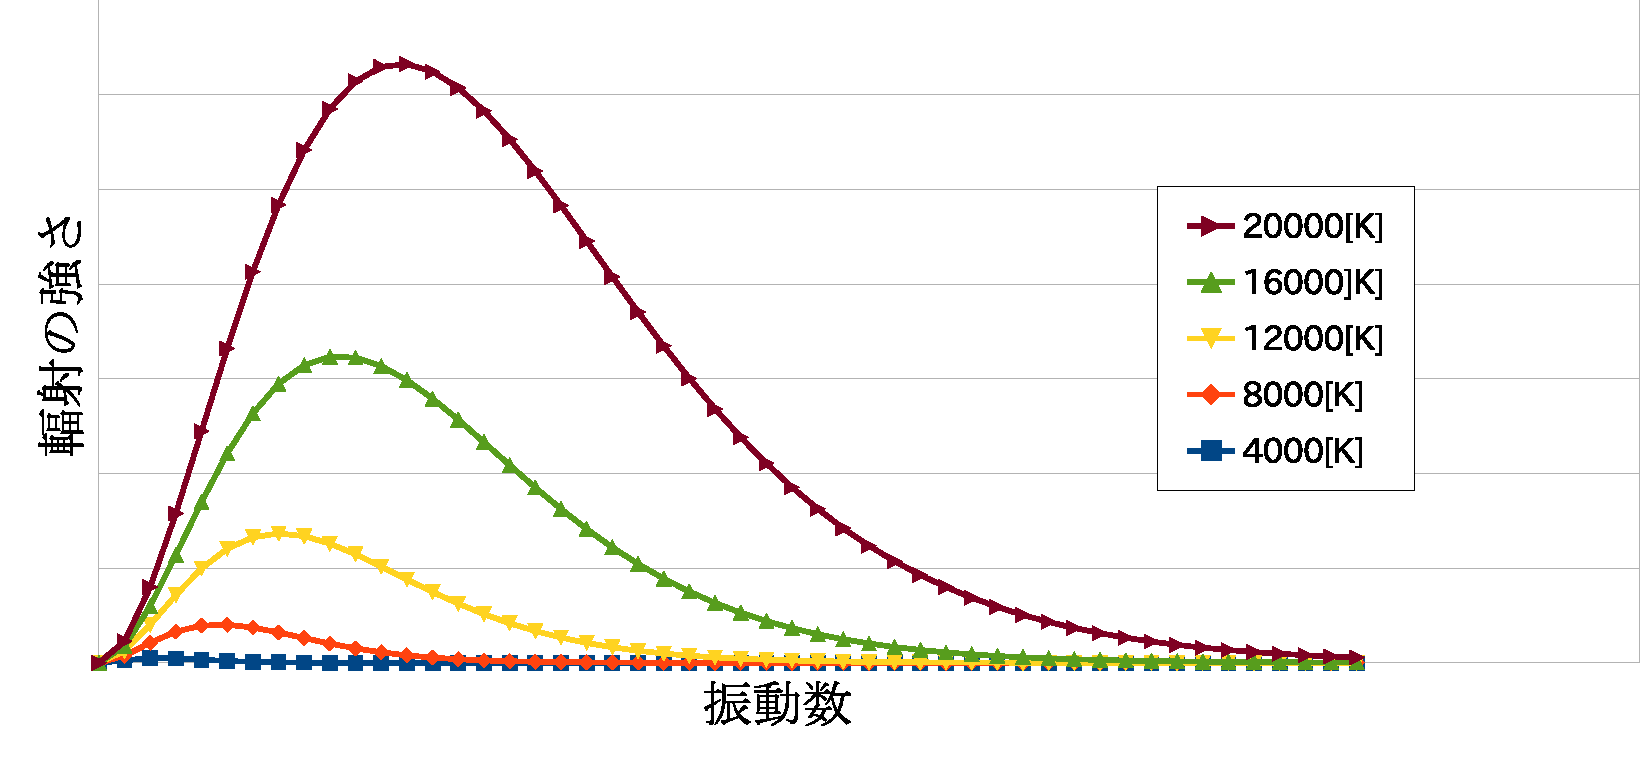
\includegraphics[keepaspectratio, width=7cm,height=4cm,clip]{PlkEq001.pdf}
                        \caption{黒体放射}
                        \label{fig:kokutai_housha_1}
                        \end{center}
                \end{figure}

            縦軸が黒体輻射の強さで,横軸が輻射される電磁波
                \footnote{
                   光とは電磁波のことであった.正確には少し違うが---というのも,可視光以外の電磁波
                   も光と言えると考えれば,電磁波であればそれは光であるとも言える.しか
                   し,光であればそれは電磁波であるとは言い切れない.光子というものが存在するから
                   である.
                }
            の周波数である.このグラフの最大値は,絶対温度によって異なり,温度が高くなるのに伴って最
            大値も上昇する.
            また,最大値となる波長は,温度が高くなるのに伴い,短くなっている.

%       %======================================================================
%       %  Subsection
%       %======================================================================
        \subsection{レイリー$=$ジーンズの公式}
            図\ref{fig:kokutai_housha_1}を完全に説明できるような式を見出すことは,困難であった.
            このグラフの比較的波長の短い部分で一致する式を1900年にレイリー
                \footnote{
                    Rayleigh
                }
            が,また1905年にジーンズ
                \footnote{
                    Jeans
                }
            が提案する.その式とは,黒体輻射のエネルギー密度を $u(\nu)$ として,
                \begin{align}
                    u(\nu)=\frac{8\pi}{c^{3}}\nu^{2}k_{B}T
                \end{align}
            である.ここで,$\mu$ は輻射される電磁波の周波数であり,
            $k_{B}$ はボルツマン定数,また $T$ は絶対温度である.
            この式は,\textbf{レイリー$=$ジーンズの公式} とよばれる.
            式の導出は,熱力学理論に従って導出される式ではあるのだが,
            黒体放射の高周波領域においては,この式で説明することはできない.
            ここに,熱力学の破綻がみられる.

%       %======================================================================
%       %  Subsection
%       %======================================================================
        \subsection{ウィーンの公式}
            黒体輻射の問題に対して,スペクトル線の方程式を与え,この問題を解決しようとした.
            その方程式とは,
                \begin{align}
                    u(\nu) = A \nu^{3} \frac{1}{\exp\left({\frac{B \nu}{CT}}\right)}
                \end{align}
            という形をしている.
            ここに,$A$,$B$,$C$ は人為的に,
            実験値と一致するように選ぶ.
            定数を確定するために,低周波領域では,
            熱力学理論から導かれたレイリー$=$ジーンズの式と一致すると仮定するならば,
                \begin{equation*}
                    A = \frac{8B\pi}{c^{3}} \quad, \qquad C = {k}_{B}
                \end{equation*}
            となる.改めて書き直せば,
                \begin{align}
                    u(\nu) = \frac{8 \pi B}{c^{3}} \nu^{3} \frac{1}{\exp\left({\frac{B \nu}{{k}_{B}T}}\right)}
                \end{align}
            となる.この式は,高周波領域で実験データと一致するが,低周波領域では実験と異なる
            値を示す.

%       %======================================================================
%       %  Subsection
%       %======================================================================
        \subsection{理論式と実験値の不一致}
            レイリー$=$ジーンズの公式とウィーンの公式を見てきた.
            しかし,これらの式は,以下のように,実験値と完全には一致しない.
            \begin{itemize}
                \item レイリー$=$ジーンズの公式は,高周波数領域では発散してしまい,実験値と一致しない
                \item ウィーンの公式は,低周波領域では実験値に不一致である
            \end{itemize}

            ただし,2つの公式は完全に的外れな式とは言い切れない.以下の点で,
            実験値と一致するからである.
            \begin{itemize}
                \item レイリー$=$ジーンズの公式は,低周波数の場合には,極めて精度よく,実験値と一致する
                \item ウィーンの公式は,高周波数の場合には,極めて精度よく,実験値と一致する
            \end{itemize}

            視覚的に示したほうが,わかりやすいであろう.
            2つの公式が示すグラフと理論とのグラフの比較を,図\ref{fig:yu}に描いた.
            残念ながら,この公式は輻射される電磁波の波長の短い場合には,
            実験結果
                \footnote{
                    実験結果とは,図では Plank と書かれているデータである.
                    プロット値は.スクリプト(perl)で計算したものである.
                    現在では実験値とプランクの式に一致していることが
                    知られているため,これを実験値と表現した.
                    計算による作図では,当然のことながら実験値など表せないので,
                    理論式を使用する必要があった.
                    ここではウィーンの公式とレイリー$=$ジーンズの公式の2つの式が
                    実験値と一致しないことを,視覚的に見るためのもので,値そのもの
                    には興味がない.あくまで,不一致のイメージを図にしただけだ.
                }
            と一致していない.
                \begin{figure}[hbt]
                    \begin{center}
                        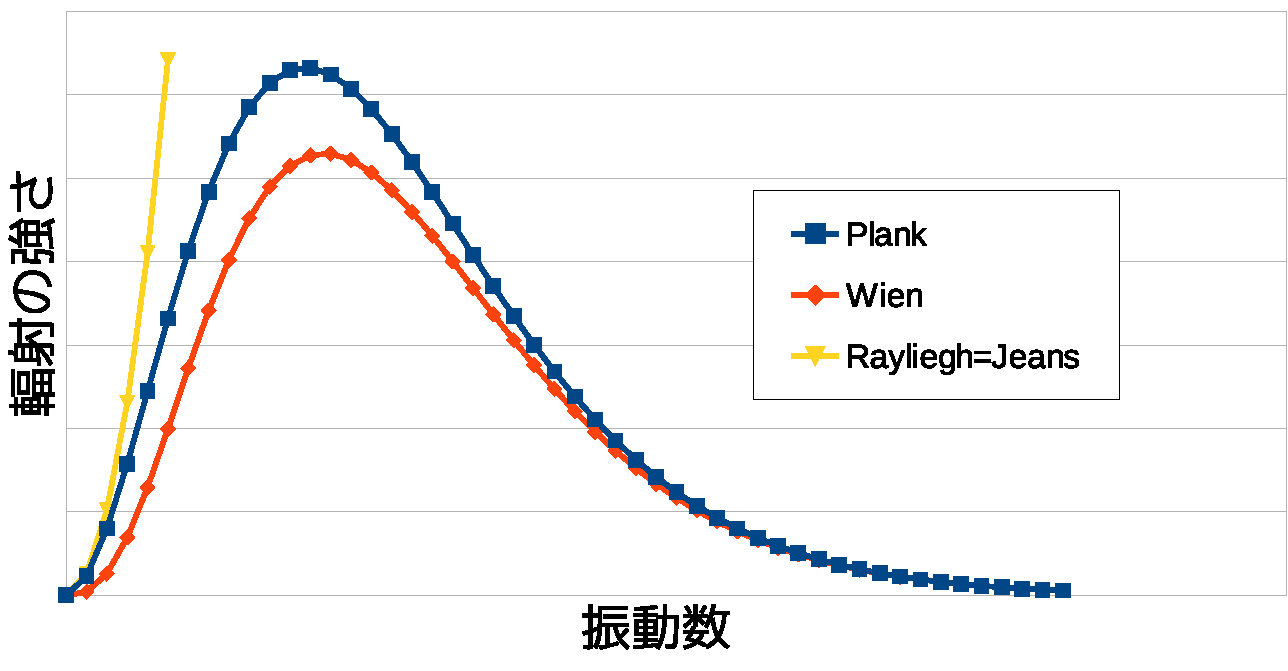
\includegraphics[keepaspectratio, width=7cm,height=4cm,clip]{BlackBoxRayleighWein.pdf}
                        \caption{各式による理論値と実験値の比較}
                        \label{fig:yu}
                    \end{center}
                \end{figure}

%       %======================================================================
%       %  Subsection
%       %======================================================================
        \subsection{プランクの式}
            プランク
                \footnote{
                    Max Karl Ernst Ludwig Planck (1858 - 1947),ドイツ
                }
            は,黒体放射の実験と一致する式を見出した.
            \begin{myshadebox}{プランクの式}
                プランクは黒体放射の強度 $u(\nu,\,T)$ と周波数 $\nu$ の の関係
                を表す式として,次式を提案した.
                    \begin{align}
                        u(\nu,\,T) = \frac{8 \pi}{{c}^{3}}
                                     {\nu}^{2}
                                     \frac{h \nu}{\exp\left( \frac{h \nu}{{k}_{B}T} \right) - 1}.
                    \end{align}

                $T$ は黒体の絶対温度,$\nu$ はそのときに放射される電磁波の周波数,$h$ はプランク定数,
                ${k}_{B}$ はボルツマン定数,$c$ は光速である.
            \end{myshadebox}

            この式は,$\nu$ が小さいときに($\nu \rightarrow 0$),レイリー$=$ジーンズの式に形を
            変える.また,$\nu$ が大きいときに($\nu \rightarrow \infty$),ウィーンの式になる.
            このことを,簡単に確認しておこう.

            \subsubsection{$1/({\e}^{x} -1)$ の極限}
            まず,次の関数の極限について知っておく必要がある.
            \begin{myshadebox}{$\displaystyle \frac{1}{\exp(x) - 1}$ の極限}
                以下の関数 $f(x)$ を考える.
                \begin{align}
                    f(x) = \frac{1}{\exp(x) - 1}
                \end{align}
                この関数は,極限に関する次の性質がある.
                \begin{align*}
                    \mbox{(1)} \quad \lim_{x \rightarrow 0} f(x) = \frac{1}{x} \quad , \qquad
                    \mbox{(2)} \quad \lim_{x \rightarrow \infty} f(x) = \frac{1}{\exp(x)}
                \end{align*}
            \end{myshadebox}

            この式の $x$ を,$x=h\nu/{k}_{B}T$ とすると,プランクの式の一部分になる.
            便宜上,一時的にその部分を,$X(\nu)$ と表そう.
            \begin{equation*}
                X(\nu) = \frac{h \nu}{\exp\left( \frac{1}{{k}_{B}T} \right) - 1 }
            \end{equation*}
            この時,以下の式が成り立つ.
            \begin{itemize}
                \item 低周波領域では,
                    $\displaystyle \lim_{\nu \rightarrow 0}      X(\nu) = \frac{{k}_{B}T}{h\nu}$ \\
                \item 高周波領域では,
                    $\displaystyle \lim_{\nu \rightarrow \infty} X(\nu) = \frac{1}{\exp\left(\frac{h\nu}{{k}_{B}T}\right)}$
            \end{itemize}

            \subsubsection{レイリー$=$ジーンズの式との関係}
            プランクの式は,この $X(\nu)$ を使うと,
            \begin{equation*}
                u(\nu,\,T) = \frac{8 \pi}{{c}^{3}} {\nu}^{2} (h \nu) X(\nu)
            \end{equation*}
            となる.
            低周波領域では,$X(\nu) = {k}_{B}T/h\nu$ であるから,
            \begin{align*}
                u(\nu,\,T) &= \frac{8 \pi}{{c}^{3}} {\nu}^{2} (h \nu) X(\nu) \\
                           &= \frac{8 \pi}{{c}^{3}} {\nu}^{2} (h \nu) \frac{{k}_{B}T}{h\nu} \\
                           &= \frac{8 \pi}{{c}^{3}} {\nu}^{2} {k}_{B}T
            \end{align*}
            と計算される.
            \begin{equation*}
                u(\nu,\,T) = \frac{8 \pi}{{c}^{3}} {\nu}^{2} {k}_{B}T
            \end{equation*}
            はレイリー$=$ジーンズの式に他ならない.

            \subsubsection{ウィーンの式との関係}
            高周波領域では,
            \begin{equation*}
                X(\nu) = \frac{1}{\exp\left(\frac{h\nu}{{k}_{B}T}\right)}
            \end{equation*}
            であるから,
            \begin{align*}
                u(\nu,\,T) &= \frac{8 \pi}{{c}^{3}} {\nu}^{2} (h \nu) X(\nu) \\
                           &= \frac{8 \pi h}{{c}^{3}} {\nu}^{3} \frac{1}{\exp\left(\frac{h\nu}{{k}_{B}T}\right)}
            \end{align*}
            ここで,$h=B$ とすれば,
            \begin{equation*}
                u(\nu,\,T) = \frac{8 \pi B}{{c}^{3}} {\nu}^{3} \frac{1}{\exp\left(\frac{B\nu}{cT}\right)}
            \end{equation*}
            となり,ウィーンの式に一致する.

%   %==========================================================================
%   %  Section
%   %==========================================================================
    \section{光の粒子性,電子の波動性}
%       %======================================================================
%       %  Subsection
%       %======================================================================
        \subsection{光は粒子としても振る舞う}
            電磁気学で学んだ通り,光は電磁波であり,従って「光は波である」と結論される.こ
            のことを,光は \textbf{波動性} の性質をもつという.
            しかし,後に示す \textbf{光電効果} という現象を観測すると,「光は波である」と
            いう主張と矛盾する部分が生じる.光電効果を観測する場合には,光は波動性ではなく
            粒子のような性質を示すのである.
            粒子のような性質のことは,光の \textbf{粒子性} とよばれる.今までの学習で常識
            的考えれば,波動性と粒子性は互いに相反する現象であり,物理現象がその性質として
            両方の性質を同時にもつものとは考えにくい.しかし,実際にそのような現象が,私達
            の馴染み深い「光」という物理現象がもっていることは事実であり,これを受け入れる
            必要がある.

%       %======================================================================
%       %  Subsection
%       %======================================================================
        \subsection{アインシュタインの光量子}
            エネルギーの変化は連続的なものではなく,離散的なものではないかとPlanckが提案をした.
            エネルギーが離散的に変化するとは,ある決まった値の整数倍の値しかとることができないということである.
            ある決まった値とは,
                \begin{align}
                    E=\nu h
                \end{align}
            である.
            アインシュタインはこのPlanckの提案を受けて,光電効果の理論的説明を与えた.アインシュタインは
            “光は粒子である”ということを仮定ば,光電効果を説明できることを示した.
            実験事実をもとに数式化したものである.
                \begin{align}
                    E=h\nu
                \end{align}
            だが,
                \begin{align*}
                    \hbar := \frac{h}{2\pi}\;,\quad\omega:= 2\pi\nu
                \end{align*}
            を導入すれば,
                \begin{align}
                    E=\hbar\omega
                \end{align}
            と書ける.

            \begin{memo}{$E=h\nu$(エネルギーと周波数の関係式)}
                $E=h\nu$の左辺であるエネルギー$E$は粒子性を表している.そして右辺の$\nu$は波動性を表す.
                つまり、この式は粒子性と波動性を関係付ける式である。この式をもう少し詳しく見ていこう.
                エネルギー順位がmからnに変化したときのエネルギーを,${E}_{m \rightarrow n}$と書こう.
                そして,このときに放出される電磁波の振動数を${\nu}_{m \rightarrow n}$とする.
                この場合の関係式は,次のとおりになる.
                \[
                    {E}_{m \rightarrow n}=h{\nu}_{m \rightarrow n}.
                \]
                これを以下のように式変形してみる.
                \[
                    \frac{{E}_{m \rightarrow n}}{{\nu}_{m \rightarrow n}} = h.
                \]
                つまり,放出されるエネルギーとそのときに発生する電磁波の比が$h$という一定の値(プランク定数)に
                なるということである.mとnは任意の自然数である
                    \footnote{
                        ただし,ここではm$>$nを想定している.
                    }.
                
            \end{memo}

%       %======================================================================
%       %  Subsection
%       %======================================================================
        \subsection{光電効果}
            レーナルト
                \footnote{
                    Philipp Eduard Anton von Lenard (1862 - 1947),ハンガリー
                }
            は光電効果を実験的に発見した.光電効果とは,簡単にいえば,金属に光を
            照射したときに,金属表面から電子が飛び出してくる現象をいう.
                        \begin{figure}[hbt]
                            \begin{center}
                                \includegraphicsdefault{kouden_kouka_image_1.pdf}
                                \caption{光電効果のイメージ}
                                \label{fig:kouden_kouka_image_1}
                            \end{center}
                        \end{figure}

            レーナルトが実験で得た光電効果の性質は3つある.すなわち,\\
                \begin{itembox}[l]{光電効果の性質}
                    \begin{enumerate}
                    \item 光電効果が起こるためには,金属表面に照射する光の周波数  $\nu$  が,
                            その金属に特有なある一定の周波数 $\nu_{0}$ より
                            大きくなければならない.この $\nu_{0}$ を \textbf{光電限界周波数} という.
                            $\nu < \nu_{0}$ だと,つまり,照射する光の周波数が $\nu_{0}$ 以下であると,
                            光電効果は起こらない.逆に,$\nu > \nu_{0}$ で
                            れば,つまり,照射する光の周波数が $\nu{0}$ より大きければ,どんなに弱い光でも,
                            光電効果は起こる.
                    \item 光電効果によって金属表面から飛び出る電子のエネルギー $E$ は,
                            光の強さに無関係であり,照射する光の周波数 $\nu$ のみ
                            によって決まる.$\nu > \nu_{0}$ の場合に,照射する光の周波数 $\nu$ と
                            飛び出す電子のエネルギー $E$ の関係は
                            \begin{align}\label{eq:Light_eq1}
                                E = h\nu -h\nu_{0}
                            \end{align}
                            で与えられる.ここに,$h$ はPlanck定数である.
                    \item 光の強さを大きくすると,金属表面から飛び出す電子の個数が増える.
                            しかし,ここの電子のエネルギーは変わらず,式(\ref{eq:Light_eq1})によって決まる.
                    \end{enumerate}
                    (阿部 龍蔵 [著],『量子力学入門』,岩波書店,2004,p31-32 を参照した.)
                \end{itembox}\\

            光電効果の関係式(\ref{eq:Light_eq1})の $h\nu_{0}$ は定数であるので,これを $W$ とおく($W=h\nu_{0}$).
            この $W$ は金属固有の値であり,各金属で異なった値をとる.$W$ を \textbf{仕事関数} という.
            また,光電効果によって金属表面から飛び出した電子のエネルギーは,もはや金属陽イオンからのクーロン力の影響
            がなく,ポテンシャルを無視できるので,運動エネルギーのみによって表現できる.飛び出す
            電子の速度を $v$,質量を $m_{e}$ としたとき,運動エネルギーは $E=(1/2)mv^{2}$ である.
            以上から,光電効果の関係式(\ref{eq:Light_eq1})は以下のように表現することもできる.
                                    \begin{align}\label{eq:Light_eq2}
                                        E &= h\nu -h\nu_{0} \notag \\
                                        \Leftrightarrow \quad \frac{1}{2}m_{e}v^{2} &= h\nu - W
                                    \end{align}
            これを,\textbf{アインシュタインの光電方程式} という.

            \begin{figure}[hbt]
                \begin{center}
                    \includegraphicsdefault{kouden_kouka_image_2.pdf}
                    \caption{光電効果(光は粒子だ!)}
                    \label{fig:kouden_kouka_image_2}
                \end{center}
            \end{figure}

%       %======================================================================
%       %  Subsection
%       %======================================================================
            \subsection{振動現象と等速円運動}
                振動現象と等速円運動についての復習をする.

                                \begin{figure}[hbt]
                                    \begin{tabular}{cc}
                                        \begin{minipage}{0.5\hsize}
                                                        \begin{center}
                                                            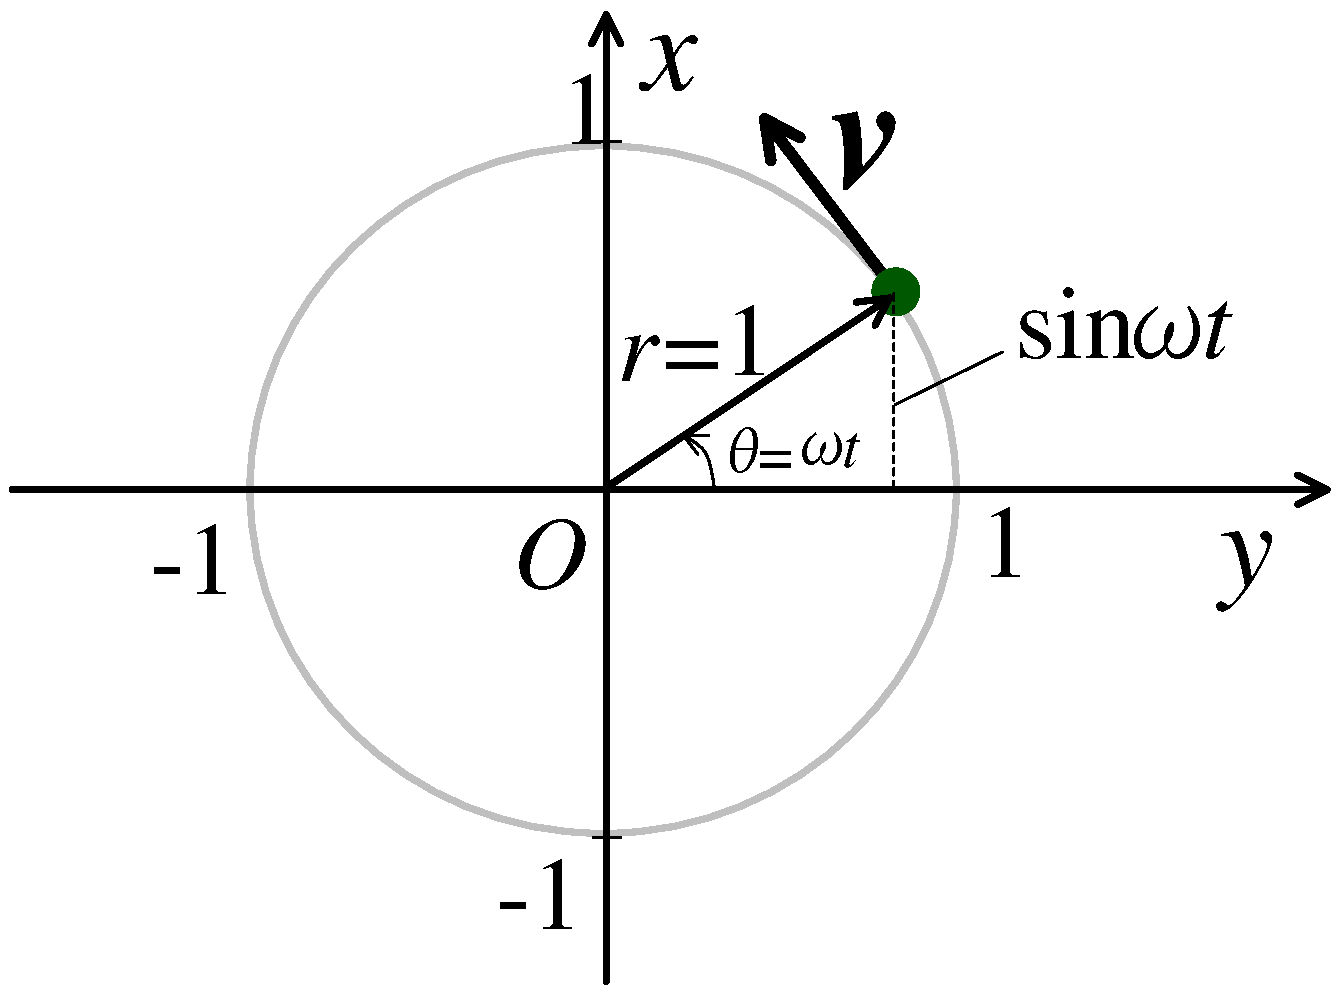
\includegraphics[keepaspectratio, width=3.4cm,height=4.2cm,clip]{enubdou2.pdf}
                                                            \caption{\ 等速円運動の関係}
                                                            \label{fig:enubdou2}
                                                        \end{center}
                                        \end{minipage}
                                        \begin{minipage}{0.5\hsize}
                                                        \begin{center}
                                                            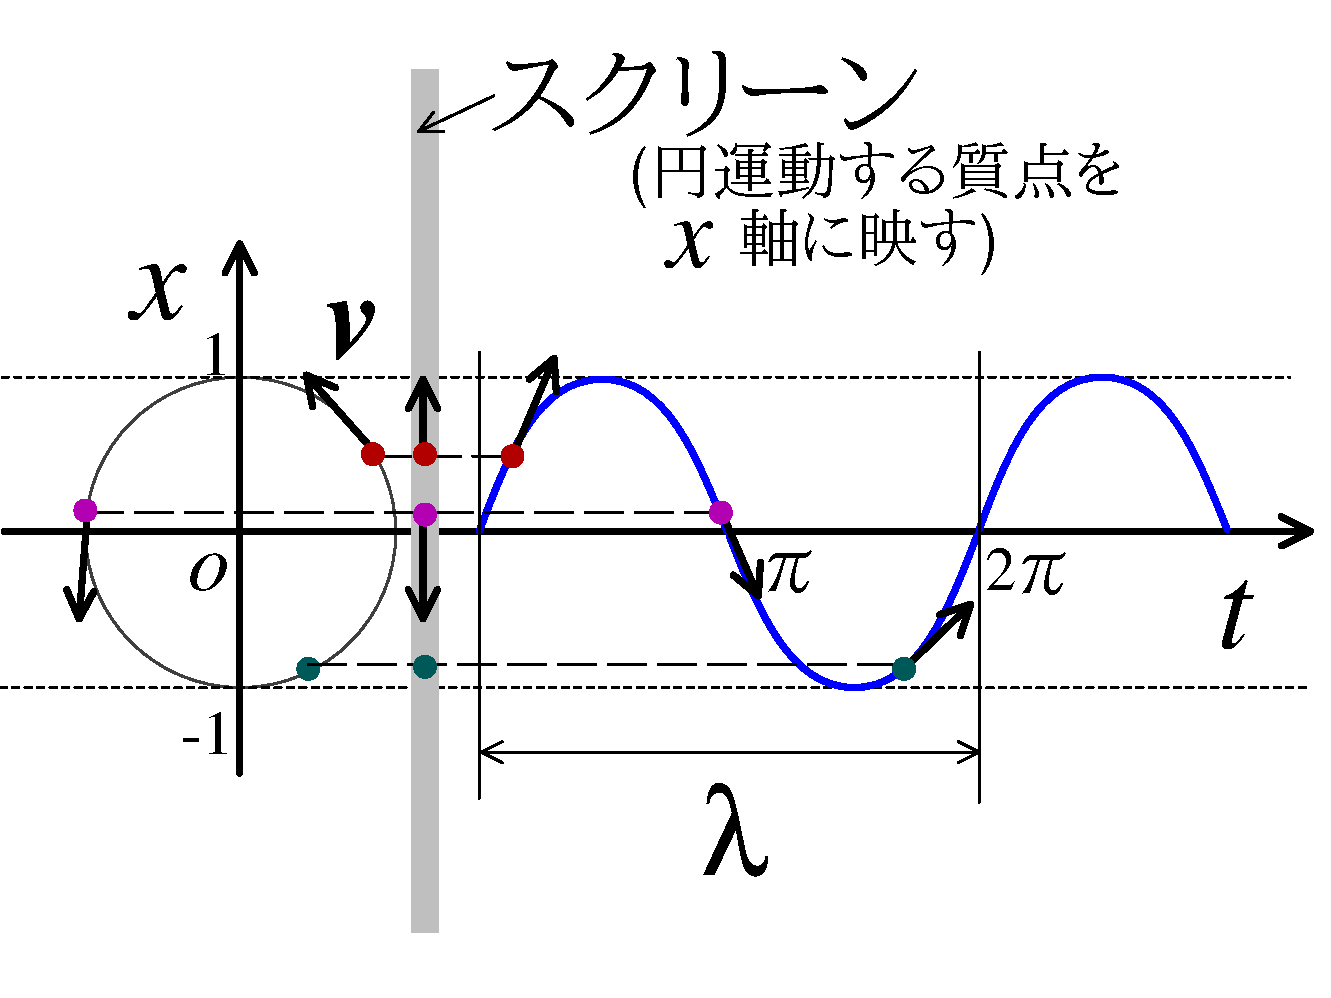
\includegraphics[keepaspectratio, width=3.4cm,height=4.2cm,clip]{enundou.pdf}
                                                            \caption{\ 単振動と等速円運動の関係}
                                                            \label{fig:enundou}
                                                        \end{center}
                                        \end{minipage}
                                    \end{tabular}
                                \end{figure}

                        まず,質点の等速円運動を考える.図\ref{fig:enubdou2}参照.半径が1である円を \textbf{単位円} という.
                        単位円の円周の長さ
                                    \footnote{
                                    半径 $r$ の円の円周の長さは $2\pi r$ である.
                                    }
                        は,$2\pi$ である.だから,この質点が単位円上を回転する速度は,
                        質点が単位円を一周するまでの時間 $T$ で円周の長さ $2\pi$ を割ればよい.
                        回転の速さのことを \textbf{角速度} ということにすれば,
                        角速度 $\omega$ は以下のように定義できる.
                            \begin{align}\label{eq:kakushuhasuu}
                                \omega=\frac{2\pi}{T}
                            \end{align}

                        さて,図\ref{fig:enundou}により,
                        質点の等速円運動の $x$ 成分だけを見ると,質点は $x$ 軸上を
                        単振動しているように見える.なぜなら,$x=\sin\omega t$ の関係があるからである.
                        この意味で,角速度は \textbf{角周波数}
                                    \footnote{
                                    定義によれば,単位円(半径 $r=1$ の円)を周期 $T=2\pi$ で
                                    一周すると,角速度が $\omega =1$ となる.
                                    }
                        とよばれることもある.
                        質点が単位円を1周するまでの時間 $T$ は単振動における \textbf{周期} に対応している
                        ことも明らかである.これからは単振動のほうを主に考えるので,
                        $\omega$ を角周波数と書き,$T$ を周期と書くことにする.


                        ところで,振動の周期 $T$ と \textbf{周波数}
                        \footnote{
                        周波数とは1[s]間における,質点の振動の回数である.
                        }
                        $\nu$ の間には,
                            \begin{align}
                                T=\frac{1}{\nu}\, \quad\left(\Leftrightarrow  \nu=\frac{1}{T} \right)
                            \end{align}
                        の関係がある.式(\ref{eq:kakushuhasuu})にこの関係式を考慮すば,
                            \begin{align}
                                \omega=2\pi\nu
                            \end{align}
                        を得る.

%           %==================================================================
%           %  Subsubsection
%           %========================s==========================================
%            \subsubsection{}
